\section{Theory}
Here is all the theory needed to understand the project.


\subsection{The physical system}
This is the section explaining the physics of the system. 
Throughout the project, \textit{natural units} are used ($\hbar = 1$,$c=1$,$e=1$,$m_e=1$) and all energies are in so-called \textit{atomix units} a.u. 

\subsubsection{The quantum mechanics and the variational principle} \label{sec:quantum_mechanics}

\paragraph{The quantum mechanics}

In this project we will look at a system of $N$ electrons in a so-called \textit{quantum dot}.
That is, a two dimensional harmonic oscillator with potential 

\eqs
V(\vec r) = \frac{1}{2} \omega^2 r^2
\label{eq:harmonic_oscillator_potential}
\eqf

This potential gives rise to a multi-particle Hamiltonian $\hat{H}$ given as the sum of an ordinary Hamiltonian and an electron repulsive part

\eqs
\hat{H} = \sum_{i=1}^N \left ( -\frac{1}{2} \nabla_i^2 + \frac{1}{2} \omega^2 r_i^2 \right ) + \sum_{i<j} \frac{1}{r_{ij}} 
\label{eq:harmonic_oscillator_hamiltonian}
\eqf

Where $r_{ij} = |\vec r_i - \vec r_j| $ is the distance between the electrons $i$ and $j$ and $r_i = |\vec r_i | = \sqrt{x_i^2 + y_i^2}$ when $\vec r_i = \left ( \begin{matrix} x_i \\ y_i \end{matrix} \right ) $. 
Our goal in this project is to find the ground eigenstate and energy of this multi-particle Hamiltonian numerically. 

\paragraph{The variational principle}\label{sec:variational_principle}

We will approach this by constructing a real test function $\Psi_T(\vec r_0, \vec r_1, ... , \vec r_{N-1}, \alpha,\beta )$ dependent on two parameters $\alpha$ and $\beta$ and calculate the expextation value of the hamilton operator $\langle \hat{H} \rangle $. 
As we know, the orthonormal eigenstates $\Psi_i$ of the Hamiltonian forms a complete basis, so any state, including our test state $\Psi_T$, can be written as a linear combination of the eigenstates 

\eqs
\Psi_T = \sum_i c_i \Psi_i
\eqf

Inserting this expression into the equation for the expectation value of $\hat{H}$ gives

\[
\langle \hat{H} \rangle = \frac{\int \Psi_T \hat{H} \Psi_T d\vec r}{ \int \Psi_T \Psi_T d\vec r} 
= \frac{\int \left ( \sum_i c_i^* \Psi_i^* \right ) \hat{H} \left ( \sum_i c_i \Psi_i \right ) d\vec r}{ \int \left ( \sum_i c_i^* \Psi_i^*  \right ) \left ( \sum_i c_i \Psi_i \right ) d\vec r}
=
\frac{\int \left ( \sum_i c_i^* \Psi_i^* \right ) \left ( \sum_i c_i  E_i \Psi_i \right ) d\vec r}{ \int \left ( \sum_i c_i^* \Psi_i^* \right ) \left ( \sum_i c_i \Psi_i \right ) d\vec r}
\]
\eqs
=
\frac{\sum_i |c_i|^2 E_i }{\sum_i |c_i|}
\eqf

The energy of the ground state $E_0$ is smaller than all other $E_i$'s so 

\eqs
\frac{\sum_i |c_i|^2 E_i }{\sum_i |c_i|} \geq \frac{\sum_i |c_i|^2 E_0 }{\sum_i |c_i|} = E_0 \frac{\sum_i |c_i|^2 }{\sum_i |c_i|} = E_0
\eqf
\eqs
\langle H \rangle \geq E_0
\eqf

This simple observation is called \textit{the variational principle} and is what we will use to narrow our search for the optimal parameters $\alpha$ and $\beta$.
We will look for the parameters $\alpha$ and $\beta$ that gives us the smallest value of $\langle \hat{H} \rangle$ and this will be our estimate for the ground state energy.







\paragraph{Finding the expectation value of $\hat{H}$}

We have

\eqs
\langle \hat{H} \rangle =  \frac{\int \Psi_T \hat{H} \Psi_T d\vec r}{ \int \Psi_T \Psi_T d\vec r}
=
\int ~\frac{\Psi_T \Psi_T}{\int \Psi_T \Psi_T d\vec r}~ \frac{1}{\Psi_T} \hat{H} \Psi_T d\vec r
\eqf

If we rename probability density function of the particles 

\eqs 
\frac{\Psi_T \Psi_T}{\int \Psi_T \Psi_T d\vec r} = P(\vec r)
\eqf

And introduce the local energy 

\eqs
E_L(\vec r) = \frac{1}{\Psi_T} \hat{H} \Psi_T
\eqf

The integral becomes 

\eqs
\langle \hat{H} \rangle = \int P(\vec r) E_L(\vec r) d\vec r = \langle E_L \rangle
\eqf

Thus, to calculate the expectation value of $\hat{H}$ we can just calculate the expectation value of the local energy.



\paragraph{Verifying that we have found an eigenstate}

We could very well find a minimum of $\langle \hat{H} \rangle$ that is not an eigen energy of the system, i.e. still larger than $E_0$.
To address this problem, let's look at the variance $V_{E_L}$ of $\langle E_L \rangle$. 

\eqs
V_{E_L} = \langle E_L^2 \rangle - \langle E_L \rangle^2
= 
\int P(\vec r) \left (\frac{1}{\Psi_T} \hat{H} \Psi_T \right )^2 d\vec r -
\left (\int P(\vec r) \frac{1}{\Psi_T} \hat{H} \Psi_T d\vec r \right )^2
\eqf 

Since

\[
\langle (E_L -\langle E_L \rangle)^2 \rangle = \langle E_L^2 - 2 E_L \langle E_L \rangle + \langle E_L \rangle^2 \rangle 
=  
\langle E_L^2 \rangle - 2 \langle E_L \rangle \langle E_L \rangle + \langle E_L \rangle^2
\]
\eqs
= \langle E_L^2 \rangle - \langle E_L \rangle^2 
=
V_{E_L}
\eqf

We have that if $V_{E_L} = 0$, then 

\eqs
\langle (E_L -\langle E_L \rangle)^2 \rangle = 0
\eqf
\eqs
0 = \int  \left (  P(\vec r) E_L(\vec r) -  \int P(\vec r) E_L (\vec r) d\vec r \right )^2 d\vec r = 
\int \left (
\frac{1}{\Psi_T} \hat{H} \Psi_T  - \int \Psi_T \hat{H} \Psi_T d\vec r 
\right )^2 d\vec r
\label{eq:Variance0_1}
\eqf

When the Hamiltonian acts on a real function, it gives a real function. 
And since $\Psi_T$ is real $\frac{1}{\Psi_T} \hat{H} \Psi_T  - \int \Psi_T \hat{H} \Psi_T d\vec r$ is real. 
By consequence

\eqs 
\left (
\frac{1}{\Psi_T} \hat{H} \Psi_T  - \int \Psi_T \hat{H} \Psi_T d\vec r 
\right )^2 > 0
\eqf

Which means that for the integral in equation \ref{eq:Variance0_1} to be zero, the following must be true for all $\vec r$

\eqs
\frac{1}{\Psi_T} \hat{H} \Psi_T  - \int \Psi_T \hat{H} \Psi_T d\vec r  = 0
\eqf
\eqs
\Psi_T \hat{H} \Psi_T = \int \Psi_T \hat{H} \Psi_T d\vec r 
\eqf

The right hand side of this equation is just a real number. 
Naming this number $E$ gives 

\eqs
\frac{1}{\Psi_T} \hat{H} \Psi_T = E 
\eqf
\eqs \hat{H}\Psi_T  = E \Psi_T  \eqf

Which is nothing but the eigenvalue equation stating that $\Psi_T$ is an eigenstate of $\hat{H}$.
This will serve as a test to see if the state we have found when minimizing the expectation value of $E_L$ is an eigenstate of the Hamilton operator. 
It is just as easily (perhaps easier) shown that if $\Psi_T$ \textit{is} and eigenstate of $\hat{H}$, then the variance of the local energy is $0$. 
This means that if the variance of our test function is \textit{not} $0$, then it is \textit{not} an eigenfunction of $\hat{H}$. 
We can summarize this discussion as follows

\eqs
\boxed{
V_{E_L} = 0 \quad \textrm{if and only if} \quad \Psi_T \textrm{ is an eigenstate of } \hat{H}
}
\eqf













\subsubsection{The test function $\Psi_T$}

We will in this project use the trial wavefunctions of $\vec r_i = \left ( \begin{matrix} x_i \\ y_i \\ \end{matrix}\right )$ given by 

\eqs
\Psi_T(\vec r_0, ... ,\vec r_{N-1})  = \Det(\phi_0,  ... , \phi_{N-1}) \cdot \textrm{J}(\vec r_0, ... , \vec r_{N-1} )
\label{eq:Trial_Wavefunction}
\eqf




\paragraph{The modified Slater determinant $\Det(\phi_0,  ... , \phi_{N-1})$}

$\Det(\phi_0,  ... , \phi_{N-1})$ is a modified \textit{Slater determinant} defined as 

\[
\Det(\phi_0,  ... , \phi_{N-1}) = |U| \cdot  |D| 
\]
\eqs
\left |
\begin{matrix}
\phi_0(\vec r_0) & \phi_2(\vec r_0) & ... & \phi_{N-2}(\vec r_0) \\
\phi_0(\vec r_2) & \phi_2(\vec r_2) & ... & \phi_{N-2}(\vec r_2) \\
       ...          &      ...       & ... & ... \\
\phi_0(\vec r_{N-2}) & \phi_2(\vec r_{N-2}) & ... & \phi_{N-2}(\vec r_{N-2}) \\
\end{matrix}
\right | \cdot 
\left |
\begin{matrix}
\phi_1(\vec r_1) & \phi_3(\vec r_1) & ... & \phi_{N-1}(\vec r_1) \\
\phi_1(\vec r_3) & \phi_3(\vec r_3) & ... & \phi_{N-1}(\vec r_3) \\
       ...          &      ...       & ... & ... \\
\phi_1(\vec r_{N-1}) & \phi_3(\vec r_{N-1}) & ... & \phi_{N-1}(\vec r_{N-1}) \\
\end{matrix}
\right |
\label{eq:Modified_Slater_Determinant}
\eqf

Where $\phi_i(\vec r_i)$ is a wavefunction resembling one of the eigenfunctions of the Hamilton operator for \textit{one} particle in a two dimensional harmonic oscillator, but parameterized by $\alpha$ in the following way:

\eqs
\phi_i(\vec r_j) = H_{n_x} (\sqrt{\alpha \omega} x_j) H_{n_y} (\sqrt{\alpha \omega} y_j) \exp(-\alpha \omega (x^2 + y^2)/2) 
\eqf


The reason for this modified version of the Slater determinant (whose real form can be explored elsewhere\footnote{\url{http://en.wikipedia.org/wiki/Slater_determinant}}) is that the spin parts of the wavefunctions are not incorporated in the expressions of $\phi_i(\vec r_j)$. 
The result is that if we were to insert these into a regular Slater determinant we would get $0$, everytime. 
The modified Slater determinant $\Det$ avoids this issue while still conserving some of the most important properties of the Slater determinant. 


$n_x(i)$ and $n_y(i)$ corresponds to the quantum numbers needed to "fill up" the system from the lowest energy levels twice (one for each spin configuration). 
For $i<12$, the explicit depence of $n_x, n_y$ on $i$ is given in table \ref{tab:dependence_of_nx_on_i}.


\begin{table}[h!]
	\centering
	\begin{tabular}{lllllllllllll}
	\toprule 
	$ i = $ & 0 & 1 & 2 & 3 & 4 & 5 & 6 & 7 & 8 & 9 & 10 & 11 \\
	\midrule
	$n_x = $ & 0 & 0 & 1 & 1 & 0 & 0 & 2 & 2 & 1 & 1 & 0 & 0 \\
	$n_y = $ & 0 & 0 & 0 & 0 & 1 & 1 & 0 & 0 & 1 & 1 & 2 & 2 \\
	\bottomrule
	\end{tabular}
	\caption{The explicit dependence of $n_x$ and $n_y$ on $i$ in the construction of the trial wavefunctions.}
	\label{tab:dependence_of_nx_on_i}
\end{table}










\paragraph{The Jastrow factor $\textrm{J} (\vec r_0, ... , \vec r_{N-1} )$} \label{sec:jastrow}

$\textrm{J} (\vec r_0, ... , \vec r_{N-1} )$ is a so-called \textit{Jastrow factor}, which represents the electron repulsion part of the wavefunction, defined as

\eqs
\boxed{
\begin{matrix} 
\textrm{J}(\vec r_0, ... \vec r_{N-1}) = \prod_{i<j}^N \exp \left (
\dfrac{a_{ij}r_{ij}}{1 + \beta r_{ij}}
\right ) 
\quad \\
\\
\textrm{where} 
\quad
r_{ij} = |\vec r_i - \vec r_j|  \quad \textrm{and} 
\quad 
a_{ij} = \left \{
\begin{matrix}
1/3  & \textrm{if spin(i) and spin(j) are parallell} \\
1  & \textrm{if spin(i) and spin(j) are anti-parallell} \\
\end{matrix}
\right .
\end{matrix}
}
\eqf

From the expression of the Jastrow factor, we see that it is zero whenever $r_{ij} = 0$ for any pair $i\neq j$. 
This is what we want from such a factor, namely that the wavefunction is zero whenever there is no distance between two particles (i.e. $r_{ij} = 0$).















\paragraph{Motivation} \label{sec:motivation}

The motivation of such a trial wavefunction is that it is partly made of the unperturbed harmonic oscillator ground states. 
See figure \ref{fig:psi_levels}. 

\begin{figure}[h!]
	\centering 
	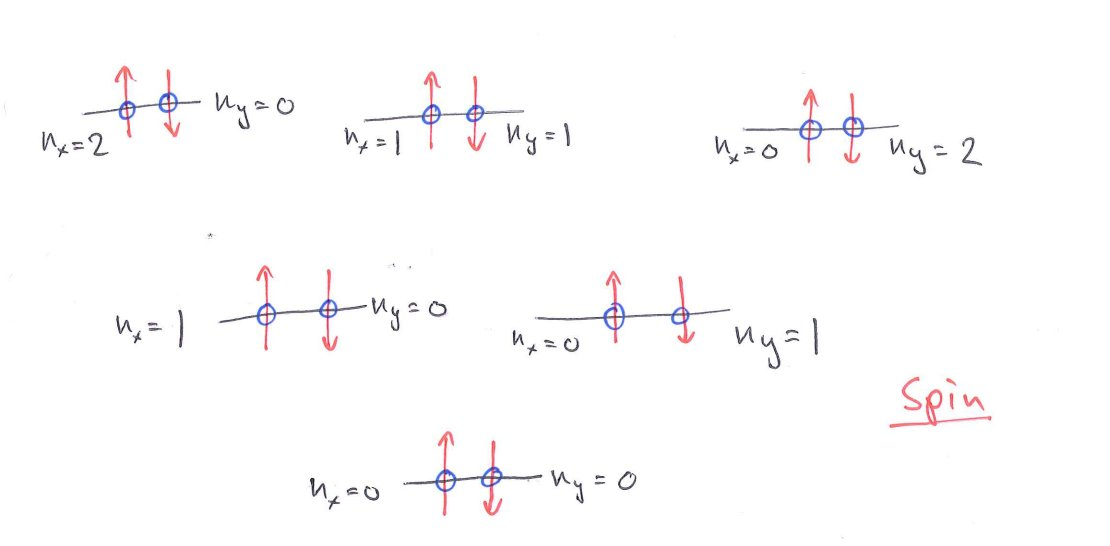
\includegraphics[width=\textwidth]{theory/psi_levels.jpg}
	\caption{The wave function levels. The blue dots represent electrons filling up the states from $n_x = n_y = 0$ to the third lowest states. 
	2 electrons fill up the lowest level, 6 electrons the two lowest levels and 12 electrons all three first energy levels.
	The net spin of each level must be $0$ due to the Pauli Exclusion principle. }
	\label{fig:psi_levels}
\end{figure}


The energies of these levels are given by the well known 2D-harmonic oscillator energy formula

\eqs
E_{n_x, n_y} = \hbar \omega (1 + n_x + n_y)
\eqf

So if we have two electrons in the lowest state ($n_x = n_y = 0$), we would expect the energy of this state to be 

\eqs
2 \cdot \hbar \omega (1 + 0 + 0) = 2 \hbar \omega = 2 \omega 
\eqf

When using natural units.

To have two electrons in the same state, their spin must be opposite due to the Pauli exclusion principle. 
This means that the total spin of the $n_x = n_y = 0$ state is $0$. 
It can be shown that the wavefunction given by equation \ref{eq:Trial_Wavefunction} when $N=2$ (i.e. two electrons) is given by the following equation

\eqs
\Psi_T (\vec r_0, \vec r_1) = \exp(-\alpha \omega (r_0^2 +r_1^2)/2) \cdot \J
\eqf

If we do not include the repulsion part of the system, there is no need to include the Jastrow Factor (for details, see section \ref{sec:jastrow}). 
It can be shown that this state is an eigenstate of the unperturbed harmonic oscillator with energy $2\omega $ when $\alpha = 1$. 
This analogy can be extended to the $N=6$ and $N=12$ electron case as well. 
When $N=6$ the unperturbed energy should be the sum of the energies in the first level (i.e. $2 \omega$) and the collective energies of the electrons in the second level states ($n_x=1,~n_y =0 \vee n_x=0,~n_y=1$) which is $4\cdot 2 \omega = 8\omega $, resulting in a total energy of $10 \omega$. 
Equivalently, the energy for the $N=12$ electron case should be $28 \omega$.
These energies will all serve as benchmarks and we should get the exact results when there is no repulsion, $\alpha = 1$ and the jastrow factor is omitted.


















\paragraph{Closed form expression of the local energy} \label{sec:closed_form_local_energy}

To evaluate the local energy 

\eqs
E_L(\vec r) = \frac{1}{\Psi_T} \hat{H} \Psi_T
=
\frac{1}{\Psi_T} \left ( 
\sum_i -\frac{1}{2}\nabla_i^2 + \sum_i V(\vec r_i) 
\right ) \Psi_T
= 
\sum_i V(\vec r_i) - \frac{1}{2} 
\sum_i \frac{1}{\Psi_T} \nabla_i^2 \Psi_T
\eqf

We need a lot of computational power. 
This is mainly due to the fact that we need to compute the sum of the laplacian operators on each particle. 
This is an easy task to do "brute force", but if we were able to find an analytical expression for the local energy, it would possibly simplify calculations by alot. 
Let's look at one of the terms in the laplacian sum, naming it $LSP$ (Laplacian sum part)

\eqs
LSP = \frac{1}{\Psi_T} \nabla_i^2  \Psi_T
\eqf

Inserting the trial wavefunction expression (equation \ref{eq:Trial_Wavefunction}) into the latter gives 

\eqs
\frac{1}{\Psi_T} \nabla_i^2  \Psi_T = \frac{1}{\Det \J} \nabla_i^2 (\Det \J)
\eqf

The function $\Det$ is a product of two matrice-determinants $|U|$ and $|D|$ where $|U|$ handles all the particles assigned spin up and $|D|$ the ones assigned spin down. 
Particle $i$ has either spin up or down, so let $|S_i|$ denote the matrix determinant which handles particle $i$ and $|S_{j\neq i}|$ denote the one that doesn't, then

\eqs
\frac{1}{\Psi_T} \nabla_i^2  \Psi_T = 
\frac{1}{|S_i| |S_{j\neq i}| \J} \nabla_i^2(|S_i| |S_{j\neq i}| \J)
=
\frac{1}{|S_i| |S_{j\neq i}| \J} |S_{j \neq i}|  \nabla_i^2(|S_i| \J)
= 
\frac{1}{|S_i| \J}  \nabla_i^2(|S_i| \J)
\eqf

Using the product rule of the laplacian operator gives 

\eqs
\boxed{
\frac{1}{\Psi_T} \nabla_i^2  \Psi_T = 
\frac{\nabla_i^2 |S_i|}{|S_i|} + \frac{\nabla_i^2 \J}{\J} + 2 \frac{\nabla_i \J}{\J} \cdot \frac{\nabla_i |S_i|}{|S_i|}
}
\eqf


It is possible to find analytical expression for all these terms, and that has been already been done in a master thesis written by Jørgen Høgberget \cite{master}. 
The arguments will not be repeated but the results are as follows 
(with names added for code reference)

\begin{subequations}
\begin{empheq}[box=\widefbox]{gather}
NSS = \frac{\nabla_i |S_i|}{|S_i|} = \sum_{k=0}^{N/2} \left [ (S^{-1})_{ki} \cdot \nabla_i \phi_{2k} (\vec r_i) \right ] \\
N2SS =\frac{\nabla_i^2 |S_i|}{|S_i|} = \sum_{k=0}^{N/2} \left [ (S^{-1})_{ki} \cdot  \nabla_i^2 \phi_{2k}(\vec r_i) \right ] \\ 
NJJ = \frac{\nabla_i \J}{\J} =   \sum_{k\neq i} \frac{a_{ik}}{r_{ik}} \frac{\vec r_i - \vec r_k}{(1 + \beta r_{ik})^2} \\
N2JJ = \frac{\nabla_i^2 \J}{\J} = \left | \frac{\nabla_i J}{J} \right |^2 + 
\sum_{k\neq i} \frac{a_{ik}}{r_{ik}} \frac{1-\beta r_{ik}}{(1+\beta r_{ik})^3 }
\end{empheq}
\label{eq:nabla_formulas}
\end{subequations}

$ \nabla_i \phi_k (\vec r_i)$ and  $ \nabla_i^2 \phi_k(\vec r_i)$ scan be found simply by inserting and taking the derivative of the Hermite polynomials.
The explicit formulas for $\phi_k$ for $k$ in the range $0$ to $11$ is given in table \ref{tab:phi_nabla} and are also taken from the master thesis by Jørgen Høgberget. 

\begin{table}[h!]
\begin{tabular}{ccccc}
	\toprule
	k & $(n_x,n_y)$ & $\phi_k(\vec r)$ & $\nabla_i \phi_k(\vec r_i) = \left [ \nabla_x, \nabla_y\right ]$ & $ \nabla_i^2 \phi_k(\vec r_i)$ \\
	\midrule
	0 & (0,0) & $1$ &  $-\left [ l^2 x ,  l^2 y\right ]$ & $l^2(l^2 r^2 - 2)$  \\ \addlinespace[0.5em]
	2 & (1,0) & $2lx$ &  $-2l \left [ (lx-1)(lx+1),l^2 xy\right ]$ & $2 l^3 x (l^2 r^2  - 4)$ \\ \addlinespace[0.5em]
	4 & (0,1) & $2ly$ &  $-2l\left [ l^2 xy,(ly-1)(ly+1)\right ]$ & $2 l^3 y (l^2 r^2 - 4) $ \\ \addlinespace[0.5em]
	6 & (2,0) & $4 l^2 x^2 - 2$ & $-2 \left [ l^2 x (2l^2 x^2 -5), l^2 y (2l^2 x^2 - 1)\right ]$ & $2 l^2(l^2 r^2 - 6 )(2 l^2 x^2 -1)$ \\ \addlinespace[0.5em]
	8 & (1,1) & $4 l^2 xy$ & $-4 l^2 \left [ y(lx-1)(lx+1),x(ly-1)(ly+1)\right ]$ & $4 l^4 xy (l^2r^2 -6)$ \\ \addlinespace[0.5em]
	10 & (0,2) &  $4 l^2 y^2 - 1$ & $- 2 \left [ l^2 x (2l^2 y^2 - 1),l^2 y (2l^2 y^2 -5)\right ]$ & $2 l^2(l^2 r^2 - 6 )(2 l^2 y^2 -1)$ \\ 
	\bottomrule
\end{tabular}
\caption{Table of derivatives of $\phi_k (\vec r_i)$ where $l=\sqrt{\alpha \omega}$.
			The factor $e^{-\frac{1}{2} l^2 r^2}$ is ommitted from all expressions.
			The formula for $k+1$ is the same as for $k$ if $k$ is even (e.g. $\phi_0 = \phi_1$).}
\label{tab:phi_nabla}
\end{table}









\subsubsection{The virial theorem}






































\subsection{The numerical foundation}
This is the section explaining the numerical theory upon which the project is built. 

\subsubsection{Monte Carlo simulations}
A Monte Carlo simulation is a way of solving a mathematical or physical problem by generating a random
(or pseudorandom
\footnote
{No electronic random number generator of today is truly random. 
The sequence of numbers generated will repeat itself after a long period. 
These periods however, are increadibly long and we will for this report 
consider the random number generators to be truly random.})
sequence of numbers and evaluating some quantity on the assumption that our the random sequence of numbers is representative of the domain from which the quantity is evaluated.
An example is evaluating the area of the unit circle by randomly placing points in a $[-1,1] \times [-1,1] $ grid and find the fraction points whose distance to the origin is $\leq 1$ and multiply this fraction by the area of the grid (i.e. $4$).
Such a simple Monte Carlo simulation can give the result as shown in figure \ref{fig:Monte_Carlo_Illustration}.

\begin{figure}[h!]
        \centering 
        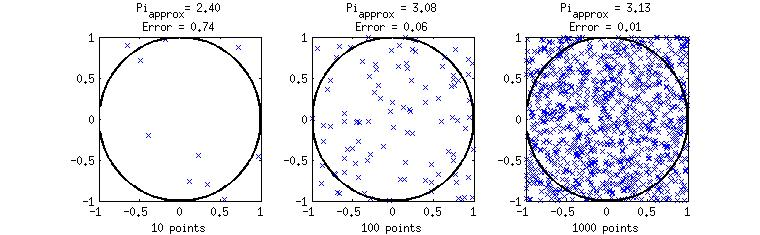
\includegraphics[width=\textwidth]{Monte_Carlo_Illustration.jpg}
        \caption{The results from a very simple Monte Carlo simulation of 
        estimating the circle constant $\pi$. 
        The precision increases with the number of points.}
        \label{fig:Monte_Carlo_Illustration}
\end{figure}

However, the method is not confined to this sort of problem, but can be applied to a variety of mathematical and physical problems. 
In this report, the method, through the Metropolis algorithm (see section \ref{sec:theory_metropolis}) has been applied to a quantum mechanical system.


\subsubsection{The Metropolis algorithm} \label{sec:theory_metropolis}

The Metropolis algorithm is a method which cleverly employs a stoichastic approach in order to quickly estimate certain mathematical objects.
The method is explained at lengths elsewhere\cite{lecturenotes}, but in this section we will look at an example which captures the main idea of the method.

Suppose we have a PDF\footnote{Probability Distribution Function} $P(x)$ in a domain $[a,b]$ for which we want to calculate the expectation value $\langle g \rangle$ of some function $g(x)$. 
The integral we need to solve is then 

\eqs
\langle g \rangle = \int_a^b P(x) g(x) dx 
\eqf

This integral can be approximated as follows

\eqs
\int_a^b P(x) g(x) dx \approx \frac{b-a}{N} \sum_i P(x_i) g(x_i) \equiv I 
\eqf

Where $x_i$ are some uniformly chosen values in the interval $[a,b]$. 
Now, imagine instead of picking values $x_i$ uniformly and weighing them by multiplying $g(x)$ with $P(x)$ instead chose the values of $\tilde{x_i}$ from the PDF $P(x)$ and calculated the quantity $\tilde{I}$ given by

\eqs
\tilde{I} = \frac{1}{N} \sum_i g(\tilde{x_i})
\label{eq:metropolis_integral}
\eqf

It can be shown mathematically that for large enough $N$, these two quantities $I$ and $\tilde{I}$ approach the same value.  
The problem with such an approach is that we need the precise expression for the PDF $P(x)$ and a robust algorithm for choosing random values from it. 
With the Metropolis algorithm however, we can use this approach \textit{without} knowing the precise expression of the PDF and the relevant values from the domain come naturally. 

The algorithm requires that we are able to calculate $\tilde{P}(x)$, an unnormalized version of $P(x)$ (i.e. some function $aP(x)$ proportional to $P(x)$). 
This may seem like a very strong requirement, but in many applications, as in this project, this is a much easier task than to calculate the precise PDF. 
The algorithm goes as follows. 
Starting with a position $x$ choose a new trial position  $x_p$ by

\eqs x_p = x + \Delta x \eqf

Where $\Delta x$ is a random step according to some rule (see subsections).
Then generate a probability criteria $s$, a random number between zero and one. 
If 

\eqs \frac{P(x_p)}{P(x)} = \frac{aP(x_p)}{aP(x)} = \frac{\tilde{P}(x_p)}{\tilde{P}(x)} \equiv w \geq s 
\label{eq:metropolis_prob_crit}\eqf

We accept the trial position as our new $x$ and if not we reject it. 
If we choose new values of $x_i$ in this manner, the collection of $x_i$'s will in fact reflect the PDF $P(x)$, which was what we needed in order to use equation \ref{eq:metropolis_integral}. 
Note how equation \ref{eq:metropolis_prob_crit} doesn't require us to have the exact form of the probability distribution function, only a function $\tilde{P}(x)$ proportional to it. 

The intuition behind the algorithm is that for each new position $x_i$ we generate is drawn towards the part of the domain where $P(x)$ is bigger. 
To see this, we note that if $P(x_p) > P(x)$ then $\frac{P(x_p)}{P(x)}>1$ which is always bigger than $s \in [0,1]$ and the new move is always accepted.
Whereas if $P(x_p)<P(x)$, the move might be rejected. 
This allows new values of $x_i$ to be chosen from where $P(x)$ is big, but at the same time allows values with lower values of $P(x)$ to be chosen. 
Which is what we expect from a PDF. 
The fact that for a large number $M$ of such steps, the values $x_i$ picked actually reflects the PDF requires some more mathematics, and once again we refer to the lecture notes of the course \cite{lecturenotes}.



\paragraph{Brute force Metropolis}

If we have no information about the physical nature of the system a reasonable way to model $\Delta x$ is the following

\eqs
\Delta x = r \Delta x_0
\eqf

Where $r$ is a random number between $0$ and $1$ and $\Delta x_0$ is a predefined step length. 
The step length $\Delta x_0$ is affecting the effectiveness of the algorithm in two contradicting ways. 
A small step length increases the probability of each suggested move $x_p$ being accepted, but weakens the ergodicity\footnote{The way in which the walker is able to reach all positions within a finite number of steps.}
of the method. 
Increasing the acceptance probability reduces the amount of times we need to evaluate the probability ratio $w$, but also increses the amount of Monte Carlo simulations needed in order to get a representative collection of $x_i$'s. 
It can be argued that a good balance between these two aspects is to achieve an acceptance ratio 
(i.e. the ratio between accepted and rejected moves) of around $0.5$. 

This is called the "Brute Force Metropolis algorithm". 

\paragraph{Importance sampling}

If our current position $x$ is in a region where the probability distribution is important, i.e. has a large value, a small step $\Delta x$ would be favorable. 
This is because we want to sample many points in this region, which is what a small step allows. 
In contrast, if the current position $x$ is in an unimportant region, we want a large step $\Delta x$ since we don't mind moving a bit farther from the region we're in. 
The brute force approach produced a step independent of the PDF value in each point, which resulted in an optimal acceptance ratio of around $0.5$. 
If we could introduce some sort of rule which adjusts the step $\Delta x$ according to the value of the PDF in the point we currently are, this could allow us to achieve an acceptance rate of around $0.9$ with the same ergodicity. 

To make such a rule, we need to use our physical understanding of the system. 
One way of doing so is to consider the points to move as a random walker would where the resulting probability is equal to the PDF we're treating.
Doing this, and invoking the Fokker-Planck and Langevin equations
\footnote{Once again we refer to the lecture notes \cite{lecturenotes} for a more detailed explanation.}
, it can be shown that the choice of $\Delta x$ is as follows

\eqs
\Delta x = DF(x) \delta t  + \eta 
\label{eq:importance_raw}
\eqf

Where $D$ is the diffusion term, $F(x)$ is a drift term which is responsible for pulling the particle towards regions where the PDF is important and $\eta$ is a gaussian random number.

Using this approach is what we will call the "Metropolis algorithm with importance sampling".


\paragraph{The metropolis algorithm for our wavefunction}
As discussed in section \ref{sec:quantum_mechanics} we need to solve the integral 

\eqs \langle E_L \rangle = \int P(\vec r) E_L(\vec r) d\vec r \eqf

Where we have a trial function 

\eqs \Psi_T(\vec r_0 ,..., \vec r_{N-1},\alpha,\beta) \eqf

dependent on 2 trial parameters $\alpha$ and $\beta$
where $\vec r_i = \left ( \begin{matrix} x_i \\ y_i \\ \end{matrix} \right )$.
This is exactly the kind of problem the Metropolis algorithm can solve and the explicit algorithm for calculating $\langle E_L \rangle$ and $\langle E_L^2 \rangle$ is given in algorithm \ref{alg:metropolis}.

\begin{algorithm}[h!]
\DontPrintSemicolon
\KwData{\;
An initial position matrix $\mathbf{r} = (\vec r_0, \vec r_1 ... \vec r_{N-1})
=
\left (
\begin{matrix}
x_0 & x_1 & ... & x_{N-1}\\
y_0 & y_1  & ... & y_{N-1}\\
\end{matrix}
\right )$ \;
A method of chosing the step $ \quad \textrm{Method}(\textbf{r}) = \Delta \vec r = \left ( \begin{matrix} \Delta x \\ \Delta y \\ \end{matrix}  \right ) $ \;}
\KwResult{\;
The expectation value of the local energy: $\langle E_L \rangle$ \;
The expectation value of the local energy squared: $\langle E_L^2 \rangle$ \;}
\Begin{
\
$\textit{cumulative\_local\_energy} = 0$ \tcp*{Initialization}
$\textit{cumulative\_local\_energy\_squared} = 0$ \;
$\textit{counter} = 0$\;
\While{$\textit{counter} < M$ }{
        $i = \textrm{randint(} 0,1,...,N-1)$ \tcp*{Choose random element index}
        $\Delta \vec r = \textrm{Method}(\mathbf{r})$
        \tcp*{Create a random two-dimensional step}
        $\mathbf{r_p} = \left ( 
        \begin{matrix} x_0 \\ y_0  \end{matrix} ~
        \begin{matrix} x_1 \\ y_1  \end{matrix} ~
        ... ~~
        \begin{matrix} x_i \\ y_i  \end{matrix} + \Delta \vec r ~~
        ... ~
        \begin{matrix} x_{N-1} \\ y_{N-1}  \end{matrix} ~
        \right ) $ \tcp*{Create a trial position matrix}
        $ s = \textrm{randint(0,1)}$ \tcp*{Generate a probability criteria}
        $w = |\psi(\alpha,\beta,\mathbf{r_p})|^2/
        |\psi(\alpha,\beta,\mathbf{r})|^2$ \tcp*{Calulate the probability ratio}
        \If{$w\geq s$}{
                $\vec r = \vec r_p$ \;
                $E_L(\mathbf{r}, \alpha, \beta) = 
                \frac{1}{\Psi_T(\mathbf{r}, \alpha, \beta)} 
                \hat{H} \psi_T(\mathbf{r},\alpha,\beta)$ \tcp*{Calculate the local energy }
                $\textit{cumulative\_local\_energy}~~ ^+_= ~~E_L(\mathbf{r}, \alpha, \beta)$ \tcp*{Update $\textit{cumulative\_local\_energy}$}
                $\textit{cumulative\_local\_energy\_squared}~~ ^+_= ~~E_L(\mathbf{r}, \alpha, \beta)^2$ \\ \tcp*{Update $\textit{cumulative\_local\_energy\_squared}$}
                $\textit{counter}~ ^+_= ~1$ \tcp*{Update \textit{counter}} 
        }       
 }
Calculate $\langle E_L \rangle = \frac{\textit{cumulative\_local\_energy}}{M}$ \;
Calculate $\langle E_L^2 \rangle = \frac{\textit{cumulative\_local\_energy\_squared}}{M}$ \;
}
\caption{The metropolis algorithm used for finding the expecation value of the
local energy and the expecation value of the local energy squared.}
\label{alg:metropolis}
\end{algorithm}

If we move only one particle at a time, each new trial position will be given by 

\eqs
\boxed{
\mathbf{r_p} = \left ( 
        \begin{matrix} x_0 \\ y_0  \end{matrix} ~
        \begin{matrix} x_1 \\ y_1  \end{matrix} ~
        ... ~~
        \begin{matrix} x_i \\ y_i  \end{matrix} + \Delta \vec r ~~
        ... ~
        \begin{matrix} x_{N-1} \\ y_{N-1}  \end{matrix} ~
        \right ) 
}
\eqf

Where $\mathbf{r} = \left ( \begin{matrix} x_0  & x_1 & ... & x_{N-1} \\ y_0  & y_1 & ... & y_{N-1} \\ \end{matrix}\right ) $. If we are using the brute force approach, then $\Delta \vec r$ is simply given by 

\eqs
\boxed{
\Delta \vec r = \Delta r \cdot \vec {\textrm{rand}}
}
\eqf

Where $\Delta r$ is a predefined step length and $\vec {\textrm{rand}}$ is a random 2-vector with elements between $-1$ and $1$. 

If we want to implement importance sampling however, we need expressions for the terms in equation \ref{eq:importance_raw}.
These terms can be shown \cite{slides} to be 

\eqs
D = \frac{1}{2}
\eqf 

Which stems from the fact that the drift is caused by kinetic energy in front of which is a factor $\frac{1}{2}$ and 

\eqs
F = 2 \frac{1}{\Psi_T}{\nabla_i \Psi_T}
\eqf

The formula for using importance sampling when choosing the trial position $\mathbf{r_p}$ for our wavefunction is thus

\eqs
\boxed{
\Delta \vec r =  \left (\frac{1}{\Psi_T } \nabla_i \Psi_T \right ) \delta t  + \eta 
}
\eqf

We can rewrite this, as in section \ref{sec:closed_form_local_energy}

\eqs
\frac{1}{\Psi_T } \nabla_i \Psi_T   = \frac{1}{|S_i| \J } \nabla_i (|S_i| \J)
=\frac{1}{|S_i| \J } \left ( |S_i| \nabla_i \J + \J \nabla_i |S_i|  \right ) 
\eqf
\eqs
\boxed{
\frac{1}{\Psi_T } \nabla_i \Psi_T  
=
\frac{\nabla_i |S_i| }{|S_i|} + \frac{\nabla_i \J}{\J}
}
\eqf

Expressions we can find both from numerical differenciation and the close form expressions in equations \ref{eq:nabla_formulas}.
In this report, we will use both these approaches and compare the CPU time needed. 

